\section{Niveau 1}

\subsection{L'implémentation}

À ce niveau du jeu, chaque usine a au plus une ressource d'entrée et de sortie. Nous avons donc décidé d'implémenter les usines de la manière suivante : 
\begin{verbatim} 
    (struct factory (consommation production cout))
\end{verbatim}

La structure \textit{factory} est composée de deux paires : une pour la consommation et une pour la production. Ainsi que d'un entier représentant le coût d'achat de la factory. Le premier élément de la paire définit le nom de la ressource et le deuxième élément le nombre de ressources consommées ou produites par unité de temps. Nous définissons donc une usine de la manière suivante : 
\begin{verbatim}
    (define wheatfact (factory (cons "wheat" 2) (cons "flour" 1) 10))
\end{verbatim}

L'usine \textit{wheat-fact} consomme deux unités de blé, produit une unité de farine et coûte 10 gold.\\
\\
\indent Ainsi, chaque chaîne de production est représentée par une liste d'usines. Nous avons donc créé la structure \textit{bench} : 
\begin{verbatim}
    (struct bench (lst-fact))
\end{verbatim}

Et enfin, la structure \textit{chain} composée d'une liste de \textit{bench}. Cette structure permet de mettre en évidence toutes les chaînes de productions créées.
\begin{verbatim}
    (struct chain (lst-bench))
\end{verbatim}

Maintenant que nous avons défini l'implémentation des usines et des chaînes de production, nous pouvons passer au parseur. 

\subsection{Le parseur}

Le parseur permet de transformer un fichier texte de donnée en une liste d'usine. \\
\indent Cependant, les fichiers textes doivent avoir un format spécial afin de pouvoir convertir ce dernier. En effet, nous prenons en compte les colonnes 1, 3 et 5 des lignes ne commençants pas par un dièse (la colonne 1 contient la consommation de l'usine, la colonne 3 la production et la colonne 5 le coût). Nous avons donc une fonction \textit{conversion} qui trie les lignes commentées et qui traduit les lignes utiles à l'aide de la fonction \textit{traduction}. 
Les chaînes de production étant implémentées, nous pouvons passer aux fonctions qui nous permettent d'implémenter la boucle du jeu.

\begin{center}
   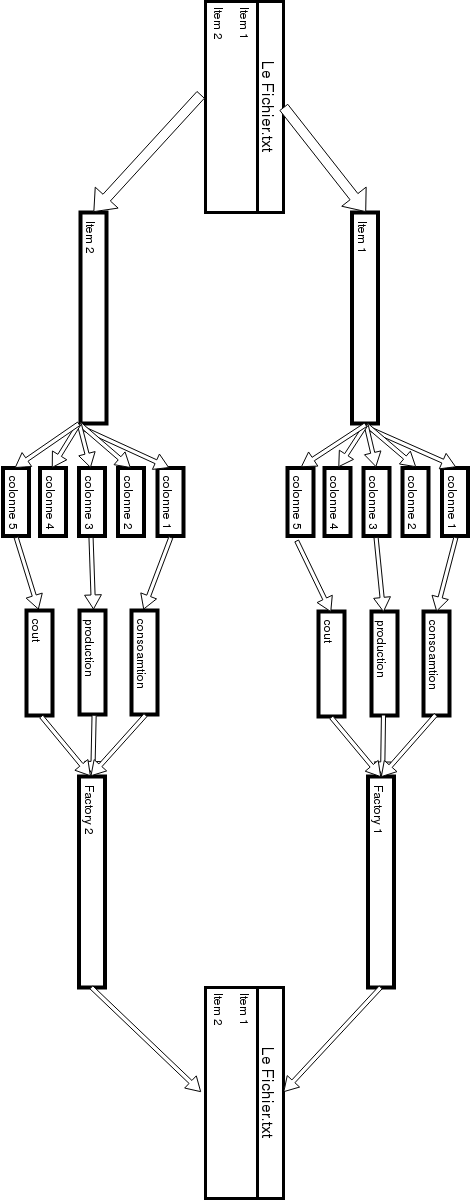
\includegraphics[scale=0.5]{parcer.png} 
\end{center}

\subsection{Tour de jeu}

On peut jouer le tour de jeu selon deux règles différentes :
\begin{itemize}
    \item La première règle qui consiste à acheter qu'une seule usine par tour.
    \item La seconde qui consiste à acheter autant d'usines que possible à chaque tour.
\end{itemize}

\subsubsection{Règle 1}

Pour pouvoir coder la fonction qui créée la boucle jeu, il suffit de connaître le gold du joueur, la chaîne de production actuelle et les achats réalisés pendant le tour. Elle retournera ensuite  le gold actuel et la chaîne de production après le tour.\\
\indent Le code sera de la forme suivante :

\begin{algorithm}[H]
\caption{tour-de-jeu-r1}
\begin{algorithmic} 
\REQUIRE $achat$
\REQUIRE $chaines$
\REQUIRE $gold$
\STATE $gold \leftarrow gold - (factory-cout achat)$ 
\STATE $add-end-rec (achat, chaines)$
\end{algorithmic}
\end{algorithm}

\indent Pour pouvoir coder le tour de jeu nous avons besoin d'une fonction auxiliaire \textit{add-end-rec} qui retournera faux et la chaîne actuelle si une usine ne peut pas être ajoutée en fin de chaîne ou vrai et la chaîne de production contenant l'usine si cette dernière peut être ajoutée. Cet algorithme sera implémenté de la manière suivante:\\


\begin{algorithm}[H]
\caption{add-end-rec}
\begin{algorithmic} 
\REQUIRE gold
\REQUIRE achat
\REQUIRE chaines
\IF{chaines vide} 
\STATE retourner faux et chaines
\ELSIF{on peut ajouter la factory à la première liste se trouvant dans chaines} \STATE retourner vrai et la chaine de production modifiée 
\ELSE 
\STATE tour de jeu (factory (cdr chaines) gold)
\ENDIF
\end{algorithmic}
\end{algorithm}

\subsubsection{Règle 2}

Pour implémenter la $2^{e}$ règle nous avons créé la fonction \textit{tour-jeu-r2} qui prend en argument le gold, la chaîne de production (\textit{chaines}) et contrairement à la règle 1, elle prend une \textit{market} qui est une liste d'usines. Nous faisons ce choix car on peut acheter autant d'usines que possible à chaque tour. Ainsi, la fonction \textit{tour-jeu-r2} est récursive. \\
\indent Elle suit le schéma suivant :\\

%oulala je comprends pas%
\indent Si \textit{add-end-rec} appliquée à gold, \textit{(car market)} et \textit{chaines} est vraie on renvoie \textit{tour-jeu-r2} appliquée au gold actuel (on soustrait le gold initial au gold de la première market car elle est achetée), à chaines modifiée à l'aide de \textit{add-end-rec} et au cdr de market. Sinon, on retourne \textit{tour-jeu-r2} au gold initial, chaines intial et (cdr market) car la première usine de market n'a pas été achetée.


\subsection{Production du Gold optimale en n tours de jeu}

Le but de cette sous-partie est d'implémenter un algorithme permettant de déterminer la quantité de Gold optimale que l'on peut produire en n tours de jeu.\\
\indent Pour cela nous avons cherché à implémenter plusieurs fonctions permettant de trouver le chemin le plus rentable. Nous avons procédé de la manière suivante : 
\begin{itemize}
    \item Tout d'abord nous extrayons dans les chaînes de production toutes les usines qui produisent du gold à l'aide de \textit{extract-factg} qui prend en argument la liste de toutes les usines que le joueur a acheté et une liste initialement vide qui sera remplie au fur et à mesure des usines qui produisent du gold.
    \item Ensuite, on enlève toutes ces usines de la liste d'origine.
    \item Enfin, on crée une forêt dont la racine de chaque arbre est une usine qui produit du gold.
\end{itemize}
\smallbreak

\indent Ainsi par exemple, considérons la chaîne de production \textit{Chaines} qui est de la forme suivante : 
\[
'((fact0 fact1 fact2) (fact3 fact2) (fact5 fact1 fact4) (fact0 fact1 fact4)) 
\]

En appliquant nos différentes fonctions à cette chaîne de production nous obtenons la forêt suivante.

\begin{figure}[H]
		\centering
		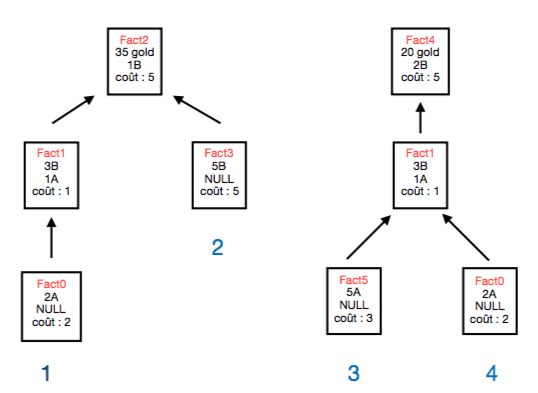
\includegraphics[scale=0.75]{factory_foret.png}
    	\caption{Forêt créée à partir de la chaîne \textit{Chaines} }
    \end{figure}


\indent Nous pouvons voir sur la FIGURE 1 qu'il y a quatre chemins possibles pour créer du gold. Ainsi, à l'aide de cette forêt nous pourrons facilement déterminer le chemin le plus rentable. \\
\smallbreak

\indent Pour trouver le meilleur chemin, nous avons implémenté la fonction \textit{best-road-tree} qui dans chaque arbre de la forêt nous indique le chemin le plus rentable. Après avoir appliqué \textit{best-road-tree} à chaque arbre, nous cherchons le meilleur chemin parmi tous les arbres. \\
\smallbreak

\indent  Reprenons l'exemple \textit{Chaines}. Nous pouvons voir ci-dessous que chaque chemin a un coût différent. 
\begin{itemize}
    \item Chemin 1 : production de 27 golds*
    \item Chemin 2 : production de 25 golds*
    \item Chemin 3 : production de 11 golds*
    \item Chemin 4 : production de 13 golds*
\end{itemize}

*\textit{après déduction des coûts de chaque usine}
\smallbreak

\indent En appliquant \textit{best-road-tree} à l'arbre de gauche, cette dernière retourne le chemin 1 et à l'arbre droit elle retourne 4. Cependant, le chemin 1 étant plus optimal que le 4 on trouve finalement que le meilleur chemin est le 1.\\


\indent Ainsi, nous pouvons voir sur cet exemple qu'il est préférable de créer des chaînes de production de la première forme pour obtenir la quantité de Gold optimal.

